\documentclass[aspectratio=169,xcolor=dvipsnames]{beamer}
\usetheme{Madrid}
\usepackage{ulem}
\usepackage{hyperref}
\usepackage{lmodern}
\usepackage{algorithm,algorithmic}
\usepackage{algorithm2e}
\usepackage{multirow}
\usepackage{listings}
\usepackage{graphicx} % Allows including images
\makeatother
\usepackage{filecontents}

% The title
\title[Optimizing C/C++]{Optimizing program performance}
\subtitle{for C/C++}

\author[Pham Ngoc Tan - Vo Khanh An]{Pham Ngoc Tan \and Vo Khanh An }
\institute[UIT] % Your institution may be shorthand to save space
{
    % Your institution for the title page
    Faculty of Computer Science \\
    University of Information Technology, VNU HCM 
    \vskip 3pt
}
\date{April, 2021} % Date, can be changed to a custom date


%----------------------------------------------------------------------------------------
%	PRESENTATION SLIDES
%------------------------0----------------------------------------------------------------

\begin{document}

%First slide
\begin{frame}
    \titlepage
\end{frame}

\begin{frame}{Reference}
    \begin{figure}
        \centering
        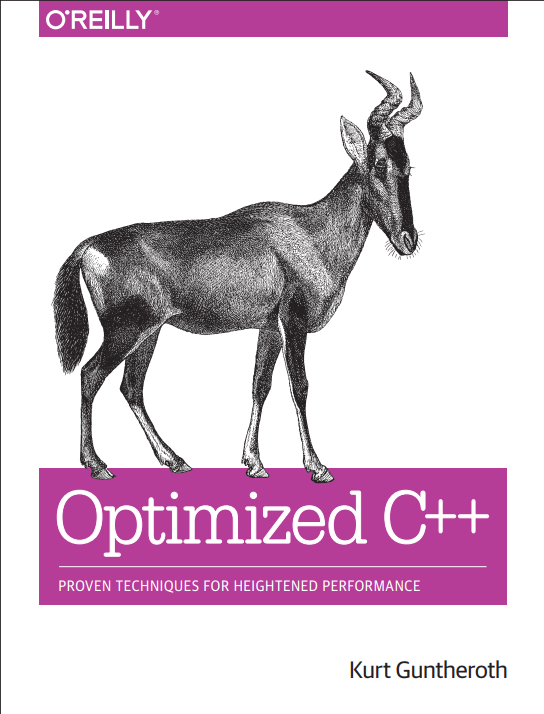
\includegraphics[scale = 0.5]{OptimizedC.png}
        \label{fig:my_label}
    \end{figure}
\end{frame}

\begin{frame}
    \frametitle{Table of Contents}
    \tableofcontents[]
\end{frame}

%Table of contents
\AtBeginSection[]
{
  \begin{frame}
    \frametitle{Table of Contents}
    \tableofcontents[currentsection]
  \end{frame}
}
\AtBeginSubsection[]
{
    \begin{frame}{Table of Contents}
        \tableofcontents[currentsection, currentsubsection]
    \end{frame}
}

\section{Introduction}
\begin{frame}{What is optimization ?}
\end{frame}
\begin{frame}{What is optimization ?}
    \begin{itemize}
        \item A coding activity
    \end{itemize}
\end{frame}
\begin{frame}{What is optimization ?}
    \begin{itemize}
        \item A coding activity
        \item Previously take place after code complete, during the integration and testing phase of a project
    \end{itemize}
\end{frame}

\begin{frame}{The goal of optimization}
\end{frame}
\begin{frame}{The goal of optimization}
    \begin{itemize}
        \item Improve the behavior of a correct program to meet customer needs\\ 
    $\Rightarrow$ As important to the development process as coding features is 
    \end{itemize}
\end{frame}

\begin{frame}{Bug fixing versus Performance tuning}
\end{frame}
\begin{frame}{Bug fixing versus Performance tuning}
\begin{itemize}
    \item Performance is a \textbf{continuous} variable  
    \item Bug is a \textbf{discrete} variable \textit{present or absent}
\end{itemize}
\end{frame}
\begin{frame}{Bug fixing versus Performance tuning}
    \begin{itemize}
        \item Performance can be either good or bad or something in between
        \item Optimization is also an iterative process in which each time the slowest part of the program is improved
    \end{itemize}
\end{frame}

\begin{frame}{Optimizing Category}
    
\end{frame}
\begin{frame}{Optimizing Category}
    When you write code for C/C++ or any programming language, your first and foremost goal is to make your program \textbf{executable} and \textbf{correct}.\\[1.0cm]
\end{frame}
\begin{frame}{Optimizing Category}
    When you write code for C/C++ or any programming language, your first and foremost goal is to make your program \textbf{executable} and \textbf{correct}.\\[1.0cm]
    After that, we consider a few things below:
\end{frame}
\begin{frame}{Optimizing Category}
    When you write code for C/C++ or any programming language, your first and foremost goal is to make your program \textbf{executable} and \textbf{correct}.\\[1.0cm]
    After that, we consider a few things below:
    \begin{itemize}
        \item Security of the program
        \item Memory consumption
        \item Speed of the program (Performance improvement)
    \end{itemize}
\end{frame}
\begin{frame}{Optimizing Category}
    When you write code for C/C++ or any programming language, your first and foremost goal is to make your program \textbf{executable} and \textbf{correct}.\\[1.0cm]
    After that, we consider a few things below:
    \begin{itemize}
        \item Security of the program
        \item \textbf{Memory consumption}
        \item \textbf{Speed of the program} (Performance improvement)
    \end{itemize}
\end{frame}

\section{Problems in Optimizing C++}    
\begin{frame}{Problems in optimizing a program}
\begin{itemize}
    \item Speed optimizing through all possible techniques, but with a tremendous memory
    \item Get conflict due to the use of 2 different optimizing goals 
\end{itemize}
\end{frame}
\begin{frame}{Problems in optimizing a program}
\begin{itemize}
    \item Speed optimizing through all possible techniques, but with a tremendous memory
    \item Get conflict due to the use of 2 different optimizing goals 
    \item Avoid cheap optimizing tricks for a better program and not receive bad consequences
    \item Despite efforts in optimizing, the program might not be completely optimized
\end{itemize}
\end{frame}
\begin{frame}{Problems in optimizing a program}
        \textit{"We should forget about small efficiencies, say about 97 percent of the time: premature optimization is the root of all evil."}
    \begin{flushright}
    \small Donald Knuth, \textit{Structured Programming with go to Statements}, ACM Computing Surveys 6(4), December 1974, p268. CiteSeerX: 10.1.1.103.6084
    \end{flushright}
\end{frame}

\begin{frame}{Ahmdal's Law}
    \begin{equation*}
        Speedup = \frac{time_{old}}{time_{new}} = \frac{1}{\left(1 - f_{cost}\right) + \frac{f_{cost}}{{f_{speedup}}}}
    \end{equation*}
\end{frame}

\begin{frame}{Ahmdal's Law}
    \begin{equation*}
        Speedup = \frac{time_{old}}{time_{new}} = \frac{1}{\left(1 - f_{cost}\right) + \frac{f_{cost}}{{f_{speedup}}}}
    \end{equation*}
s.t. 
\begin{itemize}
    \item $f_{cost}$: percentage of the program runtime used by the function $f$
    \item $f_{speedup}$: the factor to speed up $f$
\end{itemize}
\end{frame}


\begin{frame}{Ahmdal's Law}
\begin{equation*}
        Speedup = \frac{time_{old}}{time_{new}} &= \frac{1}{\left(1 - f_{cost}\right) + \frac{f_{cost}}{{f_{speedup}}}}
    \end{equation*}
If a function takes the program $40\%$ of total runtime and we have optimized it with a double speed, then the program will be $25\%$ faster 
\begin{equation*}
    Speedup = \frac{1}{\left(1 - f_{cost}\right) + \frac{f_{cost}}{{f_{speedup}}}} &= \frac{1}{\left(1-0.4\right) + \frac{0.4}{2}} = 1.25
\end{equation*}
\end{frame}

\begin{frame}{Ahmdal's Law}
\begin{itemize}
    \item An infrequently code might be not a need for optimizing
    \item \textit{"Make the common case fast and the rare case correct"}
\end{itemize}
\end{frame}

\section{Models in Optimizing C/C++ Programs}
\subsection{Use Better Data Structures}
\begin{frame}{Use Better Data Structures}
\begin{itemize}
    \item Manipulation, e.g. inserting, iterating, sorting or retrieving entries, has a runtime cost depending on data structures
    \item Using different data structures make differing use of memory costs
\end{itemize}
\end{frame}
\begin{frame}{Use Better Data Structures}
    Array case:
    \begin{itemize}
        \item Fixed memory, must declare number of items 
        \item Access to a random position in $O(1)$
        \item Add/remove one element in $O(N)$
    \end{itemize}
\end{frame}
\begin{frame}{Use Better Data Structures}
    Linked list case:
    \begin{itemize}
        \item Non-fixed memory, no need to declare number of items 
        \item Access to a random position in $O(N)$
        \item Add/remove first/last element in $O(1)$
    \end{itemize}
\end{frame}

% \subsection{Optimize Algorithms}
% \begin{frame}{Optimize Algorithms}
% \begin{itemize}
%     \item Efforts in optimizing algorithms might increase program's performance impressively
%     \item Changing into a more optimized algorithms makes more difference towards the current one when there is a huge dataset
%     \item The more optimized algorithm could even work better with a small amount of data sets if we use that algorithm sufficient enough
% \end{itemize}
% \end{frame}
% \begin{frame}{Example}
% \end{frame}
% \begin{frame}{Linear search}
%     \begin{figure}
%         \centering
%         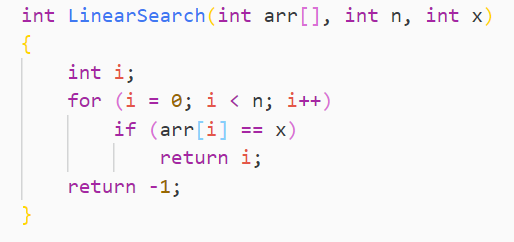
\includegraphics[scale = 1]{linearSearch.png}
%         \label{fig:my_label}
%     \end{figure}
% \end{frame}
% \begin{frame}{Linear search}
%     \begin{itemize}
%         \item $O(n)$, is expensive, but extremely general
%         \item It can be used on an unsorted table.
%         \item If the table is sorted, it’s still $O(n)$
%     \end{itemize}
% \end{frame}
% \begin{frame}{Binary search}
%     \begin{figure}
%         \centering
%         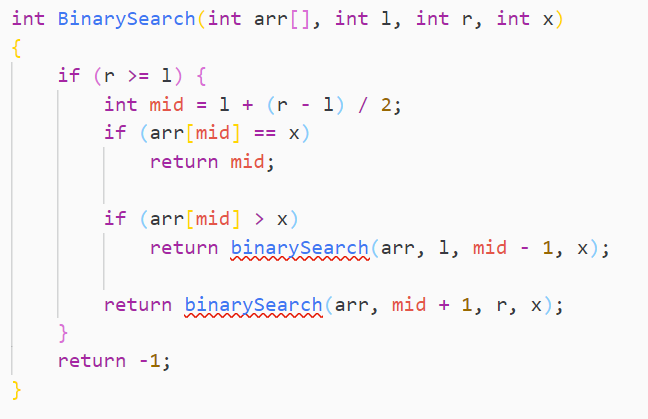
\includegraphics[scale = 1]{binarySearch.png}
%         \label{fig:my_label}
%     \end{figure}
% \end{frame}
% \begin{frame}{Binary search}
%     \begin{itemize}
%         \item $O(log_2n)$, has good performance, but it’s not the best possible search
%         \item Binary search requires input data that is sorted on the search key
%         \item Keys that can be compared not only for equality, but for an ordering relation such as less-than.

%     \end{itemize}
% \end{frame}
% \begin{frame}{Hash table}
%     \begin{figure}
%         \centering
%         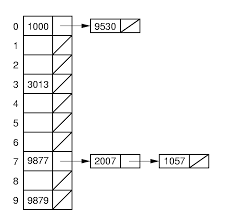
\includegraphics[scale = 0.8]{hash.png}
%         \label{fig:my_label}
%     \end{figure}
% \end{frame}
% \begin{frame}{Hash table}
% \begin{itemize}
%     \item Hashing has worst-case performance of O(n), and may
% require more hash table entries than there are records to search for. 
%     \item However, when the table has fixed contents (like month names or programming language
% keywords)\\ 
%     $\Rightarrow$ It is possible to find a record in average O(1)
% \end{itemize}
% \end{frame}
% \begin{frame}{Optimize Algorithms}
% \begin{center}
%         \begin{tabular}{|c|c|c|}
%         \hline
%             File name & Linear Search & Binary Search \\    
%         \hline
%             \multicolumn{1}{|l|}{\multirow{2}{*}{data/n1000.txt}} & Total time = 8.00991e-307 & Total time = 8.0082e-307\\
%             \multicolumn{1}{|l|}{} & Standard deviation = 0 & Standard deviation = 0\\
%             \hline
%             \multicolumn{1}{|l|}{\multirow{2}{*}{data/n10000.txt}} & Total time = 8.00991e-307 & Total time = 0.000926\\
%             \multicolumn{1}{|l|}{} & Standard deviation = 0 & Standard deviation = 9.26e-005\\
%             \hline
%             \multicolumn{1}{|l|}{\multirow{2}{*}{data/n100000.txt}} & Total time = 0.000997 & Total time = 0.00283\\
%             \multicolumn{1}{|l|}{} & Standard deviation = 9.97e-005 & Standard deviation = 0.000283\\
%             \hline 
%             \multicolumn{1}{|l|}{\multirow{2}{*}{data/n1000000.txt}} & Total time = 0.041109 & Total time = 0.020739\\
%             \multicolumn{1}{|l|}{} & Standard deviation = 0.0041109 & Standard deviation = 0.0020739\\
%         \hline 
%         \end{tabular}
%     \end{center}
%         \small \flushright
%         \text{https://github.com/vokhanhan25/Optimizing\_C/tree/master/source/optimize\_algorithm}
% \end{frame}

\subsection{Use Better Libraries}
\begin{frame}{Use Better Libraries}
    \textit{"A great library is one nobody notices because it is always there, and always has what
people need."}
    \begin{flushright}
        \small - \textbf{Vicki Myron}, author of \textit{Dewey, the Small Town Library Cat}, \\and librarian of the town of Spencer, Iowa
    \end{flushright}
\end{frame}
\begin{frame}{Use Better Libraries}
    \begin{itemize}
        \item The Standard C++ Template \textit{(STL)} is such a powerful library that it may come as surprise with its nearly-optimized speed in comparison with the others
        \item Mastering STL is a critical skill for C++ developers
        \item Benefits of this STL is that they may be use in a project instantly, which reduces coding time but sustain the quality of the project
    \end{itemize}
\end{frame}
\begin{frame}{Use Better Libraries}
    \begin{itemize}
        \item In \textit{STL}, there is a function named $sort()$ and in \textit{stdlib.h} library, there is a function named $qsort()$
    \end{itemize}
    
    
    
\end{frame}
\begin{frame}{Use Better Libraries}
    \begin{itemize}
        \item In \textit{STL}, there is a function named $sort()$ and in \textit{stdlib.h} library, there is a function named $qsort()$
        \item About comparison, the $C$  standard does not talk about complexity of $qsort()$, while the complexity of $sort()$ in the worst case is $O(NlogN)$
    \end{itemize}
\end{frame}
\begin{frame}{Use Better Libraries}
    \begin{itemize}
        \item In \textit{STL}, there is a function named $sort()$ and in \textit{stdlib.h} library, there is a function named $qsort()$
        \item About comparison, the $C$ standard does not talk about complexity of $qsort()$, while the complexity of $sort()$ in the worst case is $O(NlogN)$
        \item About runtime, STL’s $sort()$ runs $20\%$ to $50\%$ faster than the hand-coded Quick Sort and $250\%$ to $1000\%$ faster than the C $qsort()$ library function. C might be the fastest language but $qsort()$ is very slow.
    \end{itemize}
\end{frame}
\begin{frame}{Use Better Libraries}
    \begin{itemize}
        \item About flexibility, STL can work on many different data types, e.g. array, vector, deque. This flexibility is quite harder to achieve in C
    \end{itemize}
\end{frame}
\begin{frame}{Use Better Libraries}
    \begin{itemize}
        \item About flexibility, STL can work on many different data types, e.g. array, vector, deque. This flexibility is quite harder to achieve in $C$
        \item About safety, STL's $sort()$ is safer due to require no access to data via pointer as C's Standard $qsort()$ does
    \end{itemize}
\end{frame}
\begin{frame}{Use Better Libraries}
\begin{center}
        \begin{tabular}{|c|c|c|}
        \hline
            File name & qsort & sort \\    
        \hline
            \multicolumn{1}{|l|}{\multirow{2}{*}{data/n1000.txt}} & Total time = 0.000998 & Total time = 3.66937e-77\\
            \multicolumn{1}{|l|}{} & Standard deviation = 0.0002994 & Standard deviation = 3.66937e-78\\
            \hline
            \multicolumn{1}{|l|}{\multirow{2}{*}{data/n10000.txt}} & Total time = 0.010989 & Total time = 0.011042\\
            \multicolumn{1}{|l|}{} & Standard deviation = 0.001043 & Standard deviation = 0.0011042\\
            \hline
            \multicolumn{1}{|l|}{\multirow{2}{*}{data/n100000.txt}} & Total time = 0.129681 & Total time = 0.165774\\
            \multicolumn{1}{|l|}{} & Standard deviation = 0.0128718 & Standard deviation = 0.0165774\\
            \hline 
            \multicolumn{1}{|l|}{\multirow{2}{*}{data/n1000000.txt}} & Total time = 1.18596 & Total time = 1.84883\\
            \multicolumn{1}{|l|}{} & Standard deviation = 0.118497 & Standard deviation = 0.184883\\
        \hline
        \hline 
        \end{tabular}
    \end{center}
    \small \flushright
    https://github.com/vokhanhan25/Optimizing\_C/tree/master/source/use\_better\_libraries
\end{frame}

% \begin{frame}{Optimize Dynamically Allocated Variables}
%     \begin{itemize}
%         \item Almost specific features in C++ cost just a few instructions, but the cost of memory manager might costs a thousand
%         \item Copy constructors, assignments operators and input/output might take a huge cost, which is due to the association between copying and memory allocation
%     \end{itemize}
% \end{frame}
\subsection{Optimize Dynamically Allocated Variables}
\begin{frame}{Optimize Dynamically Allocated Variables}
    \begin{itemize}
        \item Except for the use of less-optimal algorithms, the naïve use of dynamically allocated variables is the greatest performance killer in C++ programs
    \end{itemize}
\end{frame}
\begin{frame}{Optimize Dynamically Allocated Variables}
    \begin{itemize}
        \item Except for the use of less-optimal algorithms, the naïve use of dynamically allocated variables is the greatest performance killer in C++ programs
        \item Improving a program’s use of dynamically allocated variables is so often that a developer can be an effective optimizer knowing nothing other than how to reduce calls into the memory manager.
    \end{itemize}
\end{frame}
\begin{frame}{Optimize Dynamically Allocated Variables}
    \begin{itemize}
        \item Except for the use of less-optimal algorithms, the naïve use of dynamically allocated variables is the greatest performance killer in C++ programs
        \item Improving a program’s use of dynamically allocated variables is so often that a developer can be an effective optimizer knowing nothing other than how to reduce calls into the memory manager.
        \item C++ to use dynamically allocated variables, like smart pointers, and strings, make writing applications in C++ productive. But there is a dark side to this expressive power 
    \end{itemize}
\end{frame}
\begin{frame}{Optimize Dynamically Allocated Variables}
    \begin{itemize}
        \item Except for the use of less-optimal algorithms, the naïve use of dynamically allocated variables is the greatest performance killer in C++ programs
        \item Improving a program’s use of dynamically allocated variables is so often that a developer can be an effective optimizer knowing nothing other than how to reduce calls into the memory manager.
        \item C++ to use dynamically allocated variables, like smart pointers, and strings, make writing applications in C++ productive. But there is a dark side to this expressive power
        \item When performance matters, $new$ is not your friend.
    \end{itemize}
\end{frame}
\begin{frame}{Create Class Instances Statically}
    \begin{figure}
        \centering
        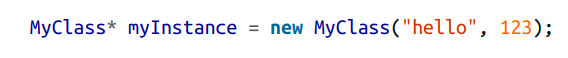
\includegraphics[scale = 0.9]{class_instance_1.png}
        \label{fig:my_label}
    \end{figure}
    \begin{figure}
        \centering
        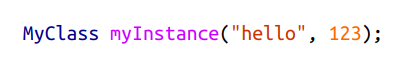
\includegraphics[scale = 0.9]{class_instance_2.png}
        \label{fig:my_label}
    \end{figure}
\end{frame}
\begin{frame}{Create Dynamic Variables Outside of Loops}
    \begin{figure}
        \centering
        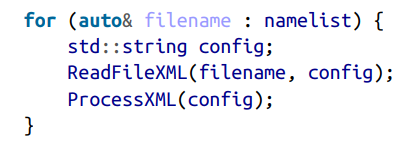
\includegraphics[scale = 0.9]{outside-1.png}
        \label{fig:my_label}
    \end{figure}
    \begin{figure}
        \centering
        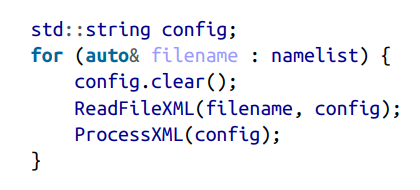
\includegraphics[scale = 0.9]{outside-2.png}
        \label{fig:my_label}
    \end{figure}
\end{frame}
\begin{frame}{Disable Unwanted Copying In The Class Definition}
    \begin{itemize}
        \item Not every object in a program should be copied 
        \item Some tremendous objects, e.g. a vector of $1,000$ strings, are brought into function meant to examine it to function properly, but the runtime cost of the copy may be considerable
        \item Forbidding copying is a must by declaring the copy constructor and assignment
operator private if copying a class is undesirable. The declaration alone is enough.

    \end{itemize}
\end{frame}
\begin{frame}{Disable Unwanted Copying In The Class Defination}
    \begin{figure}
        \centering
        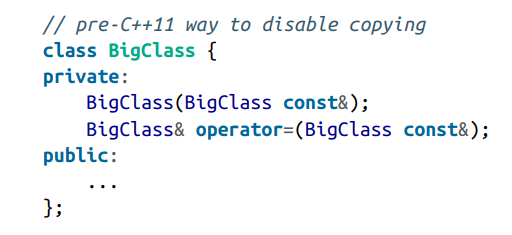
\includegraphics[scale = 0.9]{unwated_copy_1.png}
        \label{fig:my_label}
    \end{figure}
    \begin{figure}
        \centering
        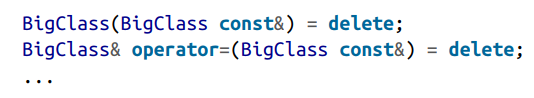
\includegraphics[scale = 0.9]{unwated_copy_2.png}
        \label{fig:my_label}
    \end{figure}
\end{frame}

\subsection{Optimize Hot Statements}
\begin{frame}{Optimize Hot Statements}
    \begin{itemize}
        \item Optimizing at the statement level can be modeled as a process of removing instructions from the stream of execution. 
        \item There is no need to focus on small-scale instructions \textit{no statement consumes more than a handful of machine instructions} $\rightarrow$ not worth
        \item We would rather find factors that magnify the cost of the statement, making it hot enough to be worth optimizing.
    \end{itemize}
\end{frame}


\begin{frame}{Remove Invariant Code from Loops}
    \begin{figure}
        \centering
        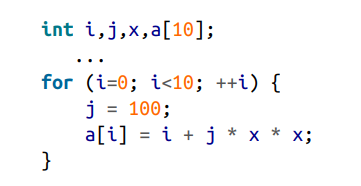
\includegraphics[scale = 0.9]{invarient_code_1.png}
        \label{fig:my_label}
    \end{figure}
    \begin{figure}
        \centering
        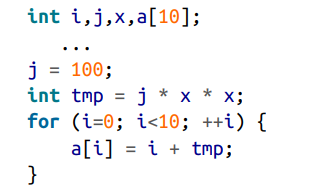
\includegraphics[scale = 0.9]{invarient_code_2.png}
        \label{fig:my_label}
    \end{figure}
\end{frame}

\begin{frame}{Optimize Hot Statements}
\begin{center}
        \begin{tabular}{|c|c|c|}
        \hline
            Iterations & Optimized & Not-optimized \\    
        \hline
            \multicolumn{1}{|l|}{\multirow{2}{*}{10000000}} & Total time = 0.225892 & Total time = 0.234375\\
            \multicolumn{1}{|l|}{} & Standard deviation = 4.3553e-6 & Standard deviation = 8.30184e-5\\
            \hline
        \end{tabular}
    \end{center}
    \small \flushright 
    https://github.com/vokhanhan25/Optimizing\_C/tree/master/source/optimize\_hot\_statements
\end{frame}

\begin{frame}{Remove Unneeded Function Calls from Loops}
    \begin{figure}
        \centering
        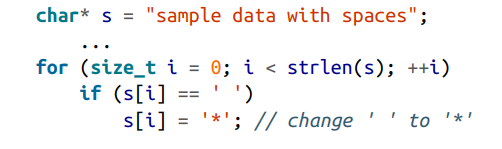
\includegraphics[scale = 0.9]{unneeded_function_1.png}
        \label{fig:my_label}
    \end{figure}
    \begin{figure}
        \centering
        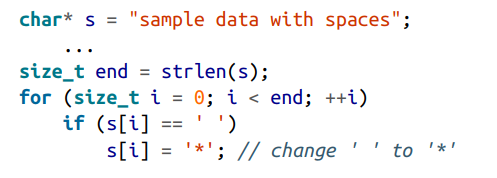
\includegraphics[scale = 0.9]{unneeded_function_2.png}
        \label{fig:my_label}
    \end{figure}
\end{frame}

\begin{frame}{Use Less Expensive Operators}
     \begin{figure}
        \centering
        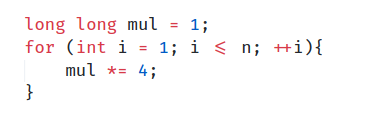
\includegraphics[scale = 0.7]{optimize_hot_statements_mul.png}
        \label{fig:my_label}
    \end{figure}
    \begin{figure}
        \centering
        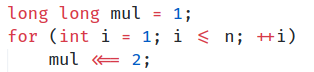
\includegraphics[scale = 0.7]{optimize_hot_statements_shift.png}
        \label{fig:my_label}
    \end{figure}
\end{frame}

\subsection{Use Better I/O}
\begin{frame}{Use Better I/O}
    \begin{itemize}
        \item Read and write are time-consuming instructions
        \item Thus, when needed, we had better use read and write from file to save time
    \end{itemize}
\end{frame}
\begin{frame}{Use Better I/O}
    \begin{figure}
        \centering
        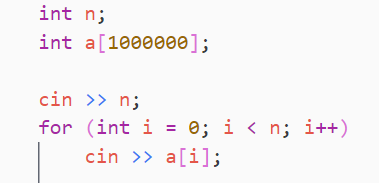
\includegraphics[scale = 0.9]{io_1.png}
        \label{fig:my_label}
    \end{figure}
    \begin{figure}
        \centering
        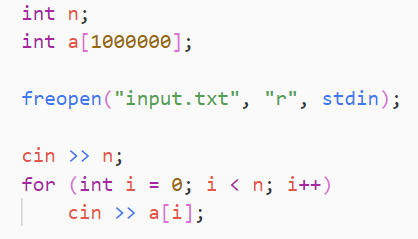
\includegraphics[scale = 0.9]{io_2.png}
        \label{fig:my_label}
    \end{figure}
\end{frame}

\subsection{Optimize Searching and Sorting}
\begin{frame}{Optimize Search Using $<$algorithm$>$ Header}
    \begin{itemize}
        \item Linear search: std::find()
        \item Binary search:
        \begin{itemize}
            \item std::binary$\_$search() 
            \item std::equal$\_$range()
            \item std::upper$\_$bound() and std::lower$\_$bound()
        \end{itemize}
    \end{itemize}
\end{frame}

\begin{frame}{Optimize Search Using $<$algorithm$>$ Header}
    \begin{itemize}
        \item Linear search: std::find() - returns an iterator to the first entry in a sequence container that compares equal to key.
        \item Binary search:
        \begin{itemize}
            \item std::binary$\_$search()
            \item std::equal$\_$range()
            \item std::upper$\_$bound() and std::lower$\_$bound()
        \end{itemize}
    \end{itemize}
\end{frame}

\begin{frame}{Optimize Search Using $<$algorithm$>$ Header}
    \begin{itemize}
        \item Linear search: std::find() - returns an iterator to the first entry in a sequence container that compares equal to key.
        \item Binary search:
        \begin{itemize}
            \item std::binary$\_$search() - returns a bool indicating whether a key is in a sorted table.
            \item std::equal$\_$range()
            \item std::upper$\_$bound() and std::lower$\_$bound()
        \end{itemize}
    \end{itemize}
\end{frame}

\begin{frame}{Optimize Search Using $<$algorithm$>$ Header}
    \begin{itemize}
        \item Linear search: std::find() - returns an iterator to the first entry in a sequence container that compares equal to key.
        \item Binary search:
        \begin{itemize}
            \item std::binary$\_$search() - returns a bool indicating whether a key is in a sorted table.
            \item std::equal$\_$range() - returns a pair of iterators delimiting a subsequence of the sorted sequence that contains entries equal to value
            \item std::upper$\_$bound() and std::lower$\_$bound()
        \end{itemize}
    \end{itemize}
\end{frame}

\begin{frame}{Optimize Search Using $<$algorithm$>$ Header}
    \begin{itemize}
        \item Linear search: std::find() - returns an iterator to the first entry in a sequence container that compares equal to key.
        \item Binary search:
        \begin{itemize}
            \item std::binary$\_$search() - returns a bool indicating whether a key is in a sorted table.
            \item std::equal$\_$range() - returns a pair of iterators delimiting a subsequence of the sorted sequence that contains entries equal to value
            \item std::upper$\_$bound() and std::lower$\_$bound() - return an iterator to the first entry of the table, whose key is less than/greater than our input key
        \end{itemize}
    \end{itemize}
\end{frame}

\subsection{Optimize Concurrency}
\begin{frame}{What Is Concurrency ?}
    Concurrency is the simultaneous execution of multiple threads of control. The goal of concurrency is not a reduction in the number of instructions executed or data words accessed per second. It is rather an increase in utilization of computing resources that reduces run time as measured.
\end{frame}

\begin{frame}{How concurrency makes our program run faster ?}
    \begin{itemize}
        \item Concurrency improves performance by permitting some program activities to move forward while other activities wait for an event to occur or a resource to become available.\\
        $\Rightarrow$ Allow computing resources to be utilized more
    \end{itemize}
\end{frame}

\begin{frame}{How concurrency makes our program run faster ?}
\begin{itemize}
    \item From the standpoint of optimization, the challenge of concurrency is to find enough independent task to fully utilize available computing resources, even if some tasks must wait on external events or availability of resources
\end{itemize}
\end{frame}

\begin{frame}{How concurrency makes our program run faster ?}
\begin{itemize}
    \item From the standpoint of optimization, the challenge of concurrency is to find enough independent task to fully utilize available computing resources, even if some tasks must wait on external events or availability of resources
    \item Concurrency can be provided to programs by the computer hardware, by operating systems, or by function libraries
\end{itemize}
\end{frame}

\begin{frame}{Some Forms of Concurrency}
    \begin{enumerate}
        \item Time slicing
        \item Threads
        \item Symmetric multiprocessing
        \item Simultaneous multi-threading
    \end{enumerate}
\end{frame}

\begin{frame}{Some Forms of Concurrency}
    \begin{enumerate}
        \item Time slicing:\\
        In time slicing, an operating system maintains a list of currently executing programs and system tasks, and allocates chunks of time to each program
        \item Threads
        \item Symmetric multiprocessing
        \item Simultaneous multi-threading
    \end{enumerate}
\end{frame}

\begin{frame}{Some Forms of Concurrency}
    \begin{enumerate}
        \item Time slicing
        \item Threads:\\
        Threads are concurrent streams of execution within a process that share the same memory. They synchronize by using synchronization primitives and communicate using shared memory locations.
        \item Symmetric multiprocessing
        \item Simultaneous multi-threading
    \end{enumerate}
\end{frame}

\begin{frame}{Some Forms of Concurrency}
    \begin{enumerate}
        \item Time slicing
        \item Threads
        \item Symmetric multiprocessing:\\
        The currently executing programs and system tasks can be run on any available execution unit, and the choice of execution unit may have consequences on performance.
        \item Simultaneous multi-threading
    \end{enumerate}
\end{frame}

\begin{frame}{Some Forms of Concurrency}
    \begin{enumerate}
        \item Time slicing
        \item Threads
        \item Symmetric multiprocessing
        \item Simultaneous multi-threading:\\
        Due to the fact that some processors are designed so that each hardware core has 2 registers sets and can execute 2 or more corresponding streams of instructions.
    \end{enumerate}
\end{frame}

\begin{frame}{Threads}
    \begin{itemize}
        \item The $<$thread$>$ header provides the std::thread template class, which allows a program to create thread objects around the operating system's own threading facilities.
        \item std::thread is a class for managing operating system threads. This also allows a program access to the operating system’s generally richer set of functions that act on threads.
    \end{itemize}
\end{frame}

\begin{frame}{Mutexes}
The mutex template definition is simple enough to be specialized for particular operating system-dependent native mutex classes.\\
\end{frame}
\begin{frame}{Mutexes}
The mutex template definition is simple enough to be specialized for particular operating system-dependent native mutex classes.\\
The $<$mutex$>$ header file contains 4 mutex templates:
\begin{itemize}
    \item std::mutex
    \item std::timed$\_$mutex
    \item std::recursive$\_$mutex
    \item std::recursive$\_$timed$\_$mutex
\end{itemize}
\end{frame}
\begin{frame}
\begin{center}
    \huge The end.
\end{center}
\end{frame}
\end{document}